\documentclass[german,notes,18pt]{beamer}
\mode<presentation>
%\usepackage[ngerman, english]{babel}
\usepackage[utf8]{inputenc}
\usepackage[T1]{fontenc}
\usepackage{amsmath,amsfonts,amssymb}
\usepackage{listings}
\usepackage{eurosym}
\usepackage{multirow}
\usepackage{color}
\usepackage{pdfpages}
\usepackage{graphicx}
\usepackage{wasysym}

\usepackage{tabularx}
\usepackage{color}
\usepackage{colortbl}
\usepackage{graphicx,import}
\usepackage{siunitx}
\usepackage[numbers]{natbib}
\usepackage{multirow}
\graphicspath{{Bilder/}}
%\beamertemplatenavigationsymbolsempty

\usetheme{kit}

\title{Projekt 1}
\subtitle{Arbeiten mit OpenMP und FEM}
\author{Thore Mehr, Fabian Miltenberger, Sébastien Thill}
\date{11.01.2017}
\institute{Lehrstuhl für Rechnerarchitektur und Parallelverarbeitung (ITEC)}

\definecolor{kit}{HTML}{009682}
\definecolor{darkgreen}{RGB}{0, 180, 0}
\definecolor{darkred}{RGB}{180, 0, 0}
\newcommand{\pro}{$\oplus$}
\newcommand{\contra}{$\ominus$}

\definecolor{shinygray}{RGB}{245,245,245}
\lstset{language=Java,
		keywordstyle=\color{blue}\bfseries,
		numberstyle=\color{blue},
		numbers=left,
		tabsize=4,
		xleftmargin=3.5em,
		xrightmargin=2em}

\begin{document}
	\selectlanguage{ngerman}
	
	\frame{\titlepage}
	
	\section{Gliederung}
	\begin{frame}
		\frametitle{Gliederung}
		
		\begin{enumerate}
			\item OpenMP und Tools (Aufgaben 1-2)
			\item Parallelisierung (Aufgaben 3-4)
			\item Partielle Differentialgleichungen (Aufgaben 5-6)
		\end{enumerate}
	\end{frame}

	\section{OpenMP und Tools}
	\subsection{Aufgabe 1}
	\begin{frame}
		\frametitle{Aufgabe 1 -- OpenMP}
		PI\\
		\begin{itemize}
			\item Reihnfolge der Threads nicht determinitisch
			\item Per Crital parallel langsamer als sequenziel
			\item Mit großen N und reduction Speedup nahe Kernzahl
		\end{itemize}
		Mandelbrot\\
		\begin{itemize}
			\item Speedup kleiner
			\item wegen Speicherverwaltung und Caches
		\end{itemize}
	\end{frame}

	\subsection{Aufgabe 2}
	\begin{frame}
		\frametitle{Aufgabe 2a) -- Tools}
		
		\begin{itemize}
			\item Meisten Fehler gefunden
			\item Durch Pragmas zu beheben
		\end{itemize}
	\end{frame}
	\begin{frame}
		\frametitle{Aufgabe 2b) -- Tools}
		\begin{itemize}
			\item O0-O3 sequenziell Pervormace ICC~GCC
			\item O0-O3 parallel ICC schneller
			\item ICC fast viel schneller
			\item ICC macht größeren Binary ~x2
			\item ICC fast riesiege Binary (~30kb vs 1,4MB)
			\item äußere Schleife parallel am schnellsten
		\end{itemize}
	\end{frame}
	\begin{frame}
		\frametitle{Aufgabe 2c) -- Tools}
		\begin{itemize}
			\item Mit expliziten Chunksize etwa dynamic und static gleich schnell
			\item auto Chunksize mit static langsam
			\item je weniger Arbeit, desto stärker ist der Effekt
			\item zu große Chunksize sehr langsam
		\end{itemize}
	\end{frame}
	
	
	
	\section{Parallelisierung}
	\subsection{Aufgabe 3}
	\begin{frame}
		\frametitle{Aufgabe 3 a)}
		
		\begin{itemize}
			\item Speedup $S(n)$ \\
			Der Geschwindigkeitszuwachs gegenüber einer sequentiellen Ausführung:
			\begin{equation*}
				S(n)=\frac{T(1)}{T(n)}
			\end{equation*}
			\item Efficiency $E(n)$ \\
			Beschleunigung pro Kern:
			\begin{equation*}
				E(n)=\frac{S(n)}{n}=\frac{T(1)}{n\cdot T(n)}
			\end{equation*}
		\end{itemize}
	\end{frame}

	\begin{frame}
		\frametitle{Aufgabe 3 a)}
		
		\begin{itemize}
			\item Mehraufwand $R(n)$ \\
			Durch Parallelisierung entstehender Aufwand:
			\begin{equation*}
				R(n) = \frac{P(n)}{P(1)}
			\end{equation*}
			\item Parallelindex $I(n)$ \\
			Operationen pro Zeiteinheit:
			\begin{equation*}
				I(n)=\frac{P(n)}{T(n)}
			\end{equation*}
			\item Auslastung $U(n)$ \\
			Mehraufwand pro Prozessor:
			\begin{equation*}
			U(n) = \frac{I(n)}{n} = R(n) \cdot E(n) = \frac{P(n)}{n \cdot T(n)}
			\end{equation*}
		\end{itemize}
	\end{frame}
	
	\begin{frame}
		\frametitle{Aufgabe 3 b)}
		
		Fehlerquellen durch Parallelisierung:
		\begin{itemize}
			\item Race Condition \\
			Wettlaufsituationen, das Ergebnis hängt von konkreter Ausführungsreihenfolge ab
			\item Dead Lock \\
			Verklemmung dadurch, dass Prozesse auf Freigabe von Resourcen warten, die von anderen Prozessen gehalten werden, die ebenfalls warten
			\item Bibliotheken
			\item Messeffekte
			\item Cacheeffekte
		\end{itemize}
	\end{frame}
	
	\begin{frame}
		\frametitle{Aufgabe 3 c)}
		
		\begin{table}
			\centering
			\begin{tabular}{l | p{3.5cm} p{4.5cm}}
				Beschleuniger & Parallelität & Anwenderfreundlichkeit \\
				\hline
				CPU & Niedrig & Gut \\
				GPU & Sehr hoch & Mittel \\
				FPGA & Hoch & Abhängig von Bibliotheken \\
				MIC & (Sehr) hoch & Gut
			\end{tabular}
		\end{table}
	
	\begin{itemize}
		\item \textbf{CPU}:
		Großer Instruktionssatz, Out-of-Order, selten mehr als 8 CPU Kerne, ,,gewöhnliche'' Programmierung
		
		\item \textbf{GPU}:
		Verbreitet, keine komplexen Befehle, massive Parallelität, \emph{SIMD}, \emph{CUDA} und \emph{OpenCL}.
		
		\item \textbf{FPGA}:
		Beliebige Eigenschaften, Testen von Chips, ,,multifunktionelle'' Beschleunigungskarte, \emph{OpenCL} oder spezielle Bibliotheken
		
		\item \textbf{MIC}:
		Gewöhnliche x86 Architektur, \emph{OpenMP} oder \emph{OpenCL}
	\end{itemize}
	\end{frame}

	\subsection{Aufgabe 4}
	\begin{frame}
		\frametitle{Aufgabe 4 -- Gauß-Seidel-Verfahren}
		\begin{itemize}
			\item Löst Gleichungssysteme der Form
			\begin{equation*}
			Au=h^2f
			\end{equation*}
			nach $u\in\mathbb{R}$ mit $A\in\mathbb{R}^{n\times n}$, $h\in\mathbb{R}$,$f\in\mathbb{R}^n$
			\item Bei uns: $A$, $h$ Abhängigkeit von Gitterkonstante $h$ gegeben, $f$ abhängig von Problem
			\item $A$ beschreibt Abhängigkeit eines Gitterpunkts zu 4 Nachbarpunkten\\
			$\Rightarrow$dünn besetzt
			\item Problemgröße ist $n=m\times m$, mit $m$ Seitenlänge des Gitters
			\item Iterativ, $u_{x,y}^k=u_j^k$ is $k$-te Iterierte für Gitterpunkt $x,y$ bzw. Eintrag $j$
		\end{itemize}
		
	\end{frame}
	\begin{frame}
		\frametitle{Aufgabe 4 -- Abhängigkeiten}
		
		\begin{figure}
			\def\svgwidth{0.6\textwidth}
			\small
			\input{gsv_node_dependence.pdf_tex}
		\end{figure}
		
	\end{frame}
	\begin{frame}
		\frametitle{Aufgabe 4 -- Abhängigkeiten}
		
		Nach GSV:
		\begin{equation*}
		u_j^{k+1}:=\frac{1}{a_{j,j}}(h^2f_j-\sum_{i=1}^{j-1}a_{j,1}u_i^{k+1}-\sum_{i=j+1}^{n}a_{j,i}u_i^k)
		\end{equation*}
		
		Zerfällt durch Struktur von $A$ und Rand (mit $d:=m-2$) zu:
		\begin{block}{Pseudocode}
			\small
			\texttt{double sum = h * h * f[j]; \\
			if (j \% d > 0) sum += u[j - 1];     // Linker Nachbarknoten \\
			if (j \% d < d - 1) sum += u[j + 1]; // Rechter Nachbarknoten \\
			if (j / d > 0) sum += u[j - d];     // Oberer Nachbarknoten \\
			if (j / d < d - 1) sum += u[j + d]; // Unterer Nachbarknoten \\
			u[j] = sum / 4;}
		\end{block}
	\end{frame}

	\begin{frame}
		\frametitle{Aufgabe 4 -- Abbruchkriterium}
		
		Annahme: Veränderung der Iterierten korreliert mit Abstand von Lösung
		$\rightarrow$ Breche ab, sobald Änderung von $u^k$ zu $u^{k+1}$ gering, also:
		\begin{equation*}
			\|u^{k+1}-u^k\|_{max}<\varepsilon_{Error}
		\end{equation*}
		
		Wir verwenden $\varepsilon_{Error}=\num{1e-6}$
	\end{frame}

	\begin{frame}
		\frametitle{Aufgabe 4 -- Parallelisierung}
		
		Nacheinander, zuerst alle grauen Felder, dann die weißen:
		
		\begin{figure}
			\color{black}
			\tiny
			\centering
			\definecolor{cbblack}{RGB}{160, 160, 160}
			\definecolor{cbwhite}{RGB}{255,255,255}
			\renewcommand*{\arraystretch}{3.6}
			\begin{tabular}{|c|c|c|c|c|c|c|}
				\hline
				\cellcolor{cbblack}$u^{k+1}_{1,1}$ & \cellcolor{cbwhite}$u^{k+1}_{2,1}$ & \cellcolor{cbblack}$u^{k}_{3,1}$ & \cellcolor{cbwhite}$u^{k}_{4,1}$ & \cellcolor{cbblack}$u^{k-1}_{5,1}$ & \cellcolor{cbwhite}$u^{k-1}_{6,1}$ & \cellcolor{cbblack}$u^{k-2}_{7,1}$ \\
				\hline
				\cellcolor{cbwhite}$u^{k+1}_{1,2}$ & \cellcolor{cbblack}$u^{k}_{2,2}$ & \cellcolor{cbwhite}$u^{k}_{3,2}$ & \cellcolor{cbblack}$u^{k-1}_{4,2}$ & \cellcolor{cbwhite}$u^{k-1}_{5,2}$ & \cellcolor{cbblack}$u^{k-2}_{6,2}$ & \cellcolor{cbwhite}$u^{k-2}_{7,2}$ \\
				\hline
				\cellcolor{cbblack}$u^{k}_{1,3}$ & \cellcolor{cbwhite}$u^{k}_{2,3}$ & \cellcolor{cbblack}$u^{k-1}_{3,3}$ & \cellcolor{cbwhite}$u^{k-1}_{4,3}$ & \cellcolor{cbblack}$u^{k-2}_{5,3}$ & \cellcolor{cbwhite}$u^{k-2}_{6,3}$ & \cellcolor{cbblack}$u^{k-3}_{7,3}$ \\
				\hline
				\cellcolor{cbwhite}$u^{k}_{1,4}$ & \cellcolor{cbblack}$u^{k-1}_{2,4}$ & \cellcolor{cbwhite}$u^{k-1}_{3,4}$ & \cellcolor{cbblack}$u^{k-2}_{4,4}$ & \cellcolor{cbwhite}$u^{k-2}_{5,4}$ & \cellcolor{cbblack}$u^{k-3}_{6,4}$ & \cellcolor{cbwhite}$u^{k-3}_{7,4}$ \\
				\hline
				\cellcolor{cbblack}$u^{k-1}_{1,5}$ & \cellcolor{cbwhite}$u^{k-1}_{2,5}$ & \cellcolor{cbblack}$u^{k-2}_{3,5}$ & \cellcolor{cbwhite}$u^{k-2}_{4,5}$ & \cellcolor{cbblack}$u^{k-3}_{5,5}$ & \cellcolor{cbwhite}$u^{k-3}_{6,5}$ & \cellcolor{cbblack}$u^{k-4}_{7,5}$ \\
				\hline
				\cellcolor{cbwhite}$u^{k-1}_{1,6}$ & \cellcolor{cbblack}$u^{k-2}_{2,6}$ & \cellcolor{cbwhite}$u^{k-2}_{3,6}$ & \cellcolor{cbblack}$u^{k-3}_{4,6}$ & \cellcolor{cbwhite}$u^{k-3}_{5,6}$ & \cellcolor{cbblack}$u^{k-4}_{6,6}$ & \cellcolor{cbwhite}$u^{k-4}_{7,6}$ \\
				\hline
				\cellcolor{cbblack}$u^{k-2}_{1,7}$ & \cellcolor{cbwhite}$u^{k-2}_{2,7}$ & \cellcolor{cbblack}$u^{k-3}_{3,7}$ & \cellcolor{cbwhite}$u^{k-3}_{4,7}$ & \cellcolor{cbblack}$u^{k-4}_{5,7}$ & \cellcolor{cbwhite}$u^{k-4}_{6,7}$ & \cellcolor{cbblack}$u^{k-5}_{7,7}$ \\
				\hline
			\end{tabular}
		\end{figure}
	\end{frame}

	\begin{frame}
		\frametitle{Aufgabe 4 -- Performance}
		Ermittelt auf dem $i82sn07$ Rechner mit 32 Kernen:
		\begin{table}
			\centering
			\begin{tabular}{r|r|rr|rr|@{ \dots}|rr}
				Problem & Seq. & \multicolumn{2}{c|}{2 Threads}  & \multicolumn{2}{c|@{ \dots}|}{4 Threads} & \multicolumn{2}{c}{32 Threads} \\
				$n$ & Zeit & T(2) & S(2) & T(4) & S(4) & T(32) & S(32) \\
				\hline
				225 & 0,005 & 0,007 & 0,357 & 0,008 & 0,625 & 1,361 & 0,0389 \\
				961 & 0,053 & 0,056 & 0,473 & 0,049 & 1,08 & 4,041 & 0,178 \\
				\vdots & \vdots & \multicolumn{2}{c|}{\vdots} & \multicolumn{2}{c|@{ \dots}|}{\vdots} & \multicolumn{2}{c}{\vdots} \\
				65.025 & 115 & 81 & 1,42 & 45,3 & 2,54 & 25,33 & 4,54 \\
				261.121 & 1340 & 943 & 1,42 & 504 & 2,67 & 177 & 7,57 \\
			\end{tabular}
		\end{table}
	\end{frame}
	
	
	\section{Partielle Differentialgleichungen}
	\subsection{Aufgabe 5}
	\begin{frame}
		\frametitle{Aufgabe 5 a)}
		Gegeben:
		\begin{equation*}
			-\Delta u(x,y)=f(x,y), (x,y)\in\Omega=(0,1)^2, u(x,y)=0, (x,y)\in\Gamma
		\end{equation*}
		
		Die Bedingungen:
		\begin{itemize}
			\item $\Omega$ beschränktes Gebiet
			\item $\Gamma$ hinreichend glatt
			\item $f:\Omega\rightarrow \mathbb{R}$
		\end{itemize}
	\end{frame}

	\begin{frame}
		\frametitle{Aufgabe 5 b)}
		
		Gesucht ist $f$ mit
		\begin{equation*}
		u(x,y)=\sin(2M\pi x)\sin(2N\pi y)
		\end{equation*}
		Anwendung des \emph{Laplace-Operators} $\Delta$:
		\begin{equation*}
		\small
		\begin{split}
		f(x,y)&=-\Delta u(x,y) \\
		&= -\frac{\partial u}{\partial x^2}-\frac{\partial u}{\partial y^2} \\
		&= -\frac{\partial}{\partial x}(2M\pi\cos(2M\pi x)\sin(2N\pi y)) -\frac{\partial}{\partial y}(2N\pi\sin(2M\pi x)\cos(2N\pi y)) \\
		&= 4M^2\pi^2\sin(2M\pi x)\sin(2N\pi y) + 4N^2\pi^2\sin(2M\pi x)\sin(2N\pi y) \\
		&= (M^2+N^2)4\pi^2\sin(2M\pi x)\sin(2N\pi y)
		\end{split}
		\end{equation*}
	\end{frame}

	\begin{frame}
		\frametitle{Aufgabe 5 c)}
		\vspace{-12em}
		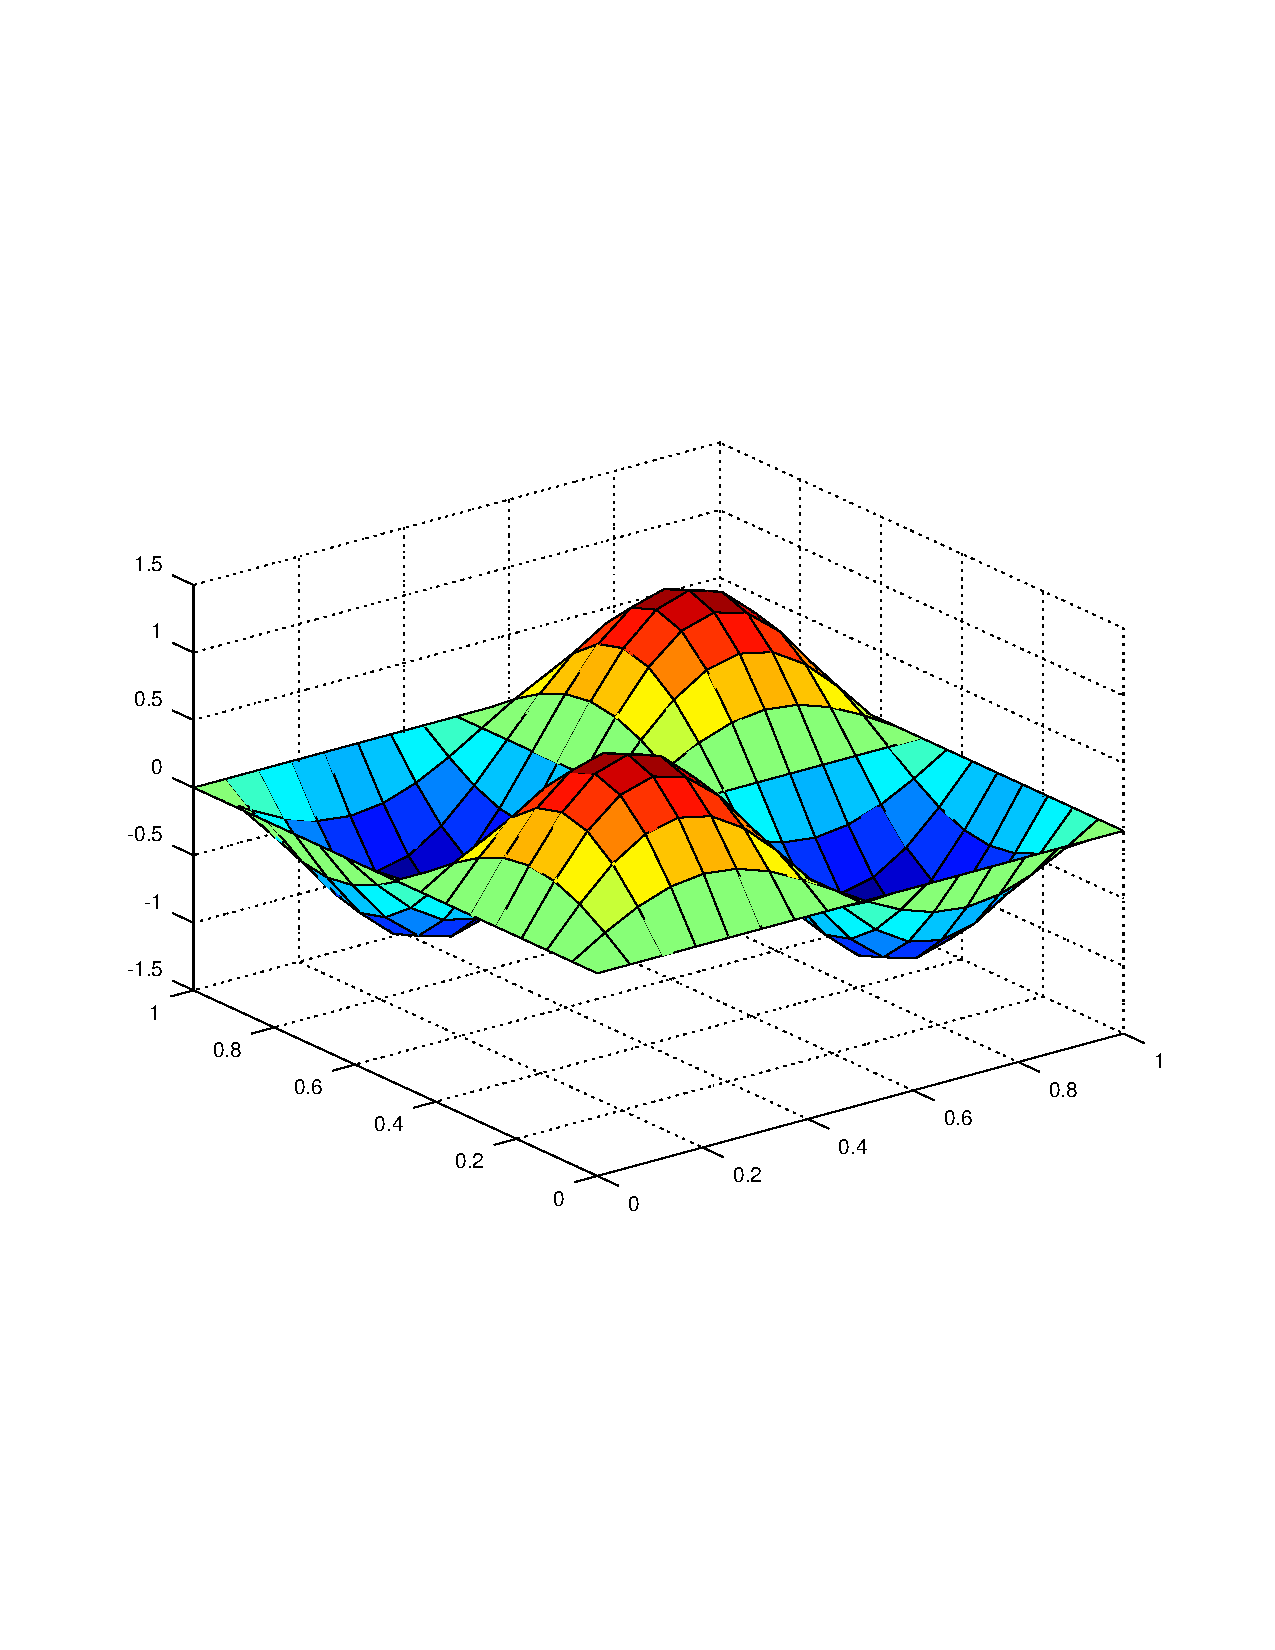
\includegraphics[width=\textwidth]{a5l3}
		\vspace{-12em}
		$l=3,h=\frac{1}{8}$
	\end{frame}

	\begin{frame}
	\frametitle{Aufgabe 5 c)}
	\vspace{-12em}
	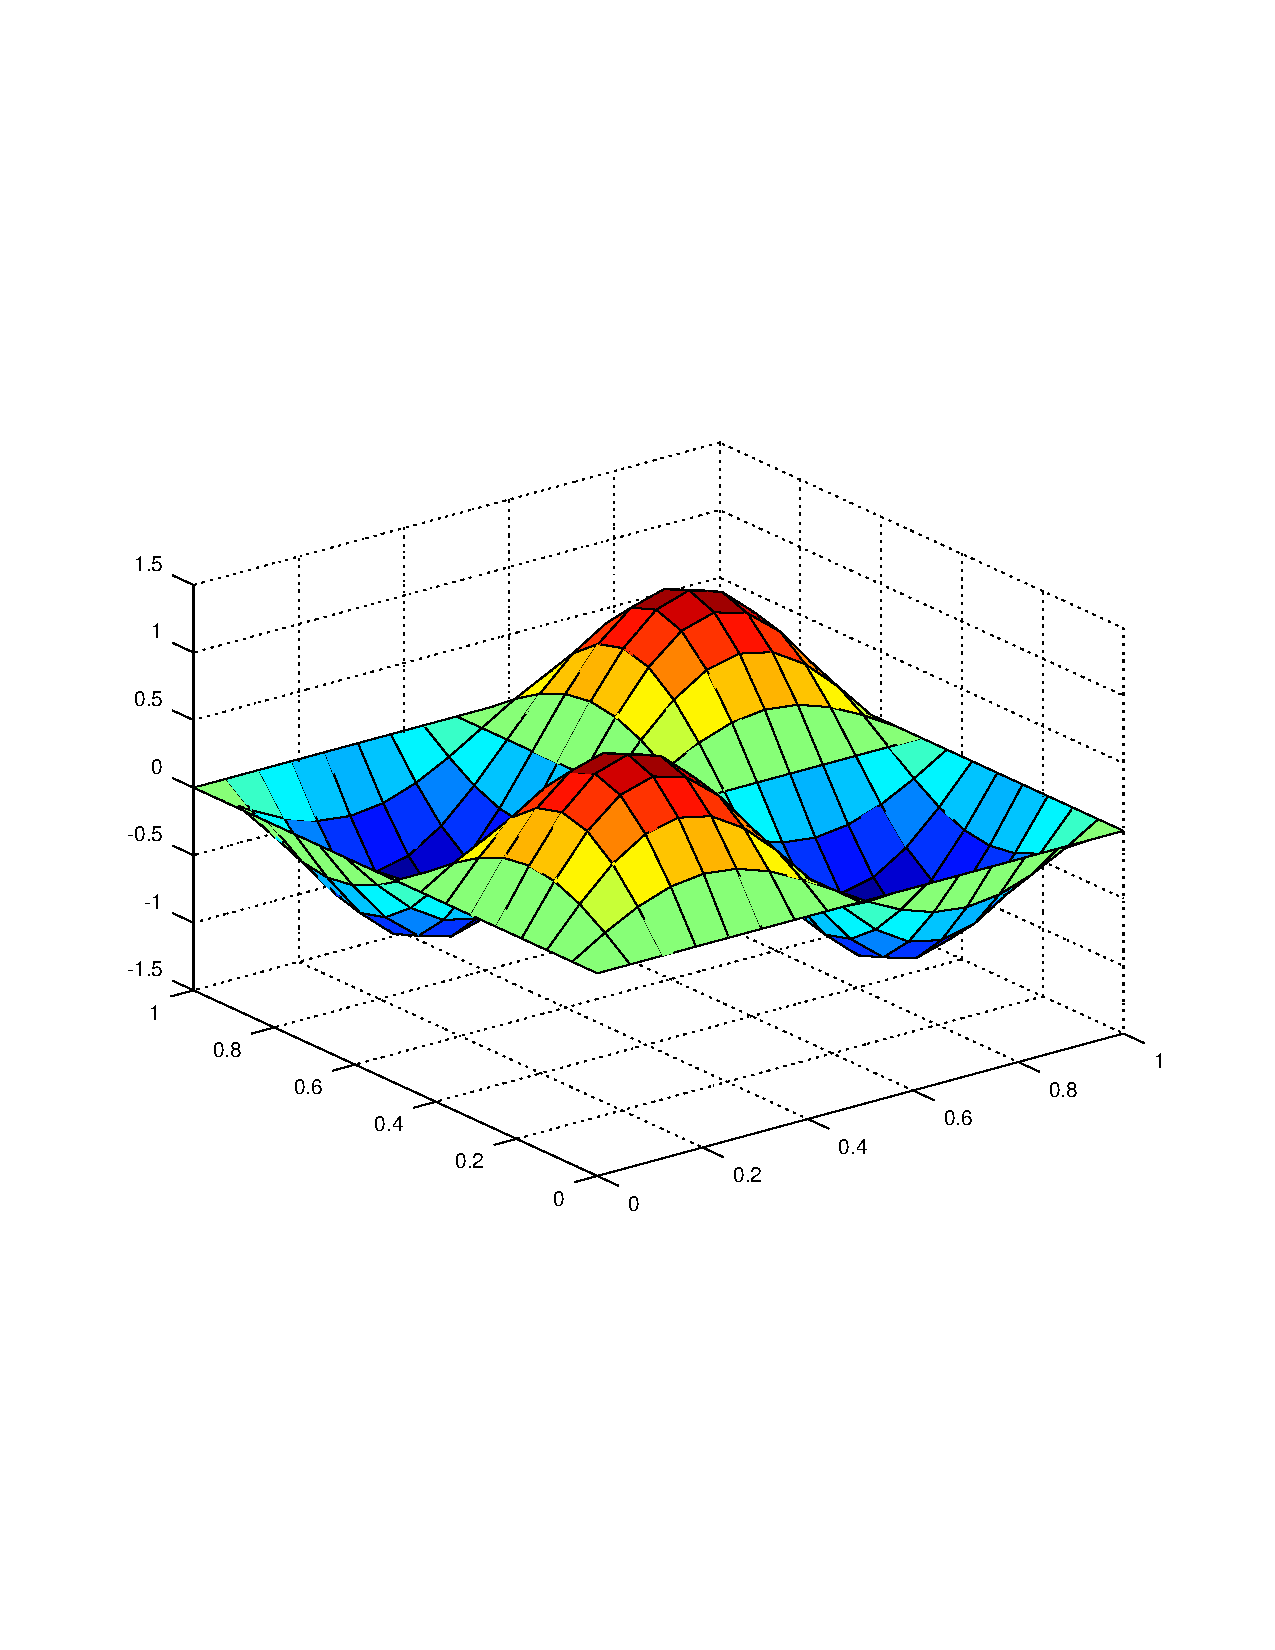
\includegraphics[width=\textwidth]{a5l4}
	\vspace{-12em}
	$l=4,h=\frac{1}{16}$
	\end{frame}
	
	\begin{frame}
	\frametitle{Aufgabe 5 c)}
	\vspace{-12em}
	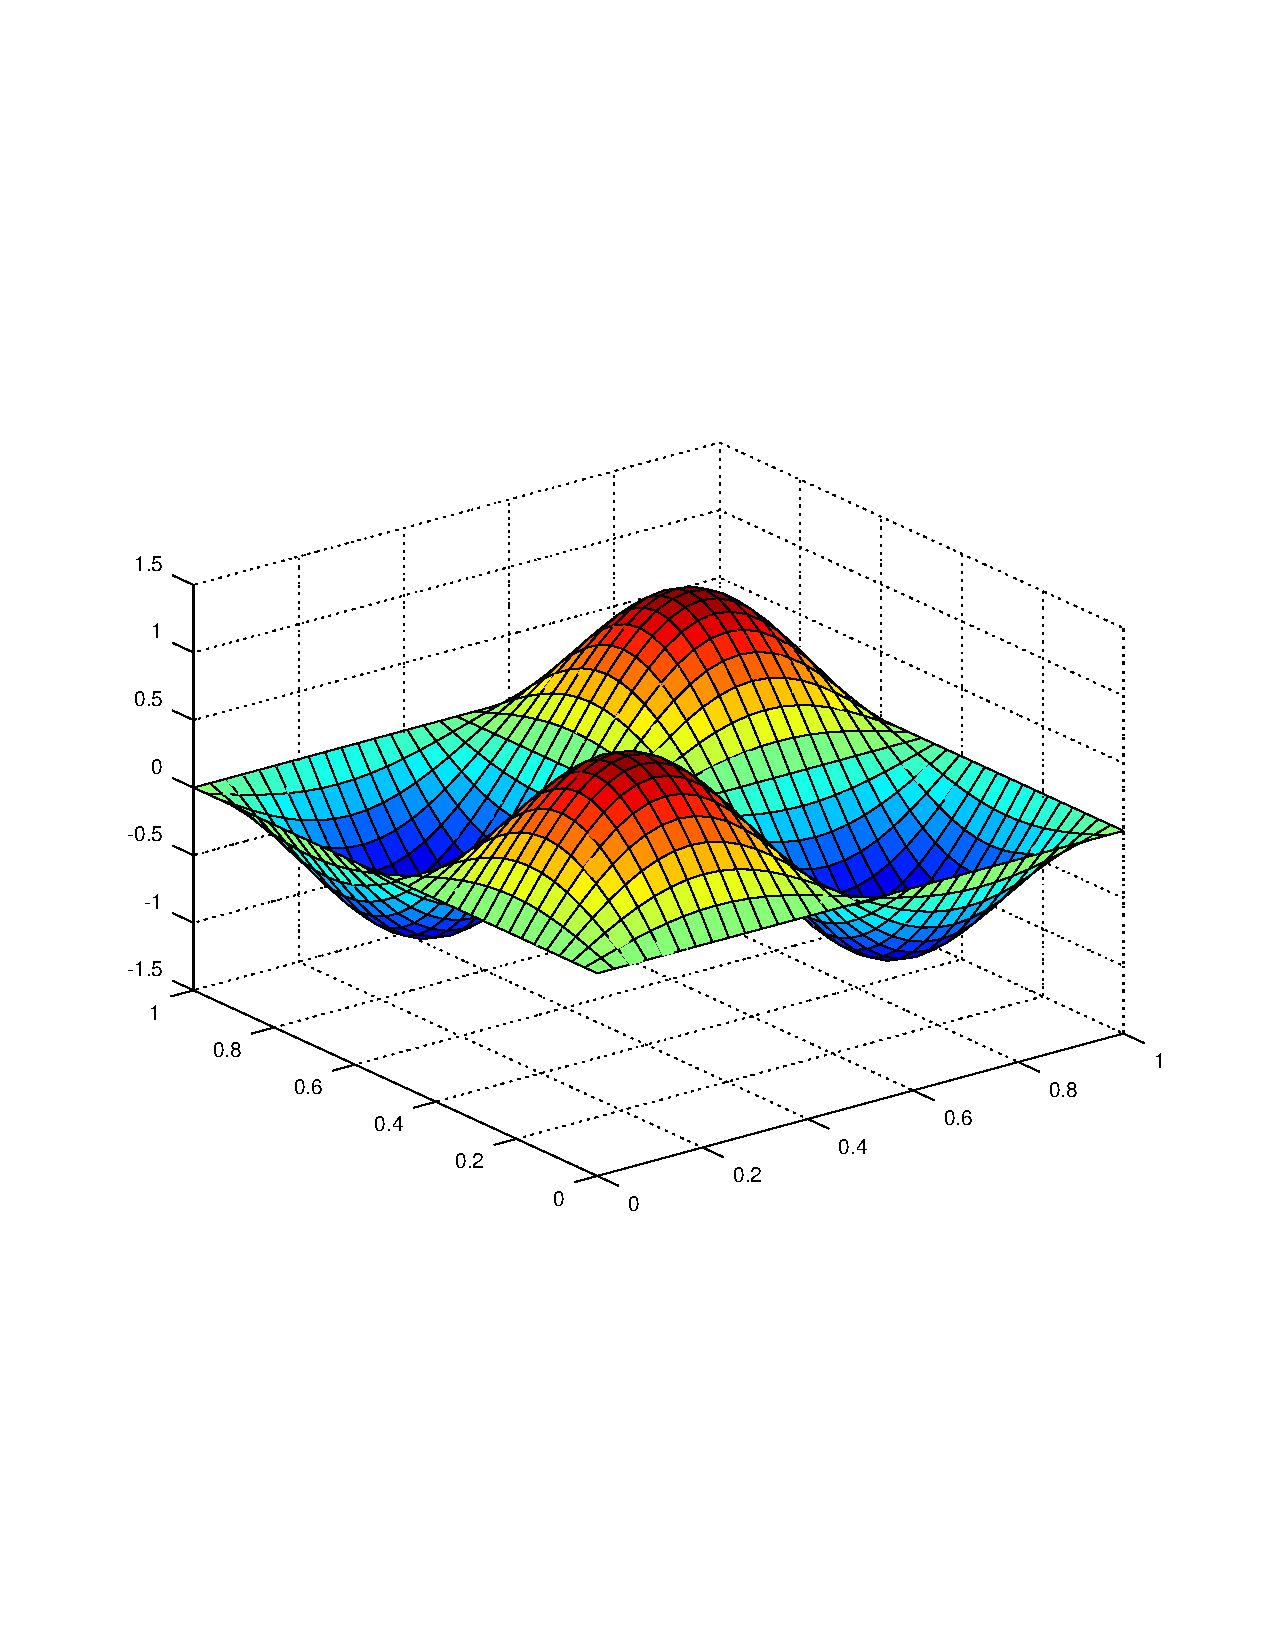
\includegraphics[width=\textwidth]{a5l5}
	\vspace{-12em}
	$l=5,h=\frac{1}{32}$
	\end{frame}

	\begin{frame}
		\frametitle{Aufgabe 5 c)}
		
		Fehler zu analytischen Lösung wird mit kleinerem $h$ kleiner\\
		$\Rightarrow$ Es handelt sich um eine \emph{h-FEM-Methodik}, da die Polynomgrade nicht verändert wurden
	\end{frame}
	
	\subsection{Aufgabe 6}
	\begin{frame}
		\frametitle{Aufgabe 6 a)}
		
		Alphabetische Liste gängiger Krylow-Unterraum-Verfahren:
		\begin{itemize}
			\item Arnoldi-Verfahren, zur Eigenwertapproximation
			\item BiCG, das CG-Verfahren für nicht SPD-Matrizen
			\item BiCGSTAB, Stabilisierung von CGS
			\item BiCGSTAB(ell), Stabilisierung von CGS
			\small
			\item BiCGSTABTFQMR, der Ansatz hinter TFQMR angewandt auf BiCGSTAB
			\footnotesize
			\item BiOres, eine Variante des BiCG-Verfahrens
			\scriptsize
			\item BiOmin, eine Variante des BiCG-Verfahrens
			\tiny
			\item BiOdir, eine Variante des BiCG-Verfahrens
			\Tiny
			\item CG, zur approximativen Lösung linearer Gleichungssysteme
			\fontsize{4pt}{0pt}\selectfont
			\item CGNE, CG-Verfahren auf den Normalgleichungen, Variante 1
			\fontsize{3pt}{0pt}\selectfont
			\item CGNR, CG-Verfahren auf den Normalgleichungen, Variante 2
			\fontsize{2pt}{0pt}\selectfont
			\item CGS-Verfahren, quadrierte BiCG-Rekursion
			\fontsize{1pt}{0pt}\selectfont
			\item FOM, zur approximativen Lösung linearer Gleichungssysteme
			\item GMRES, zur approximativen Lösung linearer Gleichungssysteme
		\end{itemize}
		\vspace{-0.5em}\hspace{3em}\vdots \\
		$\Rightarrow$ Es gibt sehr viele
	\end{frame}

	\begin{frame}
		\frametitle{Aufgabe 6 a)}
		Für uns relevant:
		\begin{itemize}
			\item CG-Verfahren \\
			Geeignet für große lineare, symmetrische, positiv definite und dünn besetzte LGS, spätestens $n$ Schritten  exakte Lösung
			
			\item GMRES \\
			Geeignet für große, dünn besetzte LGS, exakte Lösung erst nach endlich vielen Schritten
			
			\item Lanczos-Verfahren \\
			Konvergenz von Eigenwerten abhängig
		\end{itemize}
	\end{frame}

	\begin{frame}
		\frametitle{Aufgabe 6 b)}
		
		Speedup und Effizienz von \emph{CG-Verfahren} gegenüber \emph{Gauß-Seidel-Verfahren} (Problem aus Aufgabe 5)
		\begin{table}
			\centering
			\begin{tabular}{r|r|rr|@{ \dots}|rr|rr}
				Problem & Seq. & \multicolumn{2}{c|@{ \dots}|}{2 Threads} & \multicolumn{2}{c|}{16 Threads}  & \multicolumn{2}{c}{32 Threads} \\
				$n$ & S(1) & S(2) & E(2) & S(16) & E(16) & S(32) & E(32) \\
				\hline
				225 & 1,74 & 1,81 & 0,906 & 2,44 & 0,153 & 2,93 & 0,0917 \\
				961 & 4,01 & 3,71 & 1,86 & 1,44 & 0,0898 & 3,46 & 0,109 \\
				\vdots & \vdots & \multicolumn{2}{c|@{ \dots}|}{\vdots} & \multicolumn{2}{c|}{\vdots} & \multicolumn{2}{c}{\vdots} \\
				65.025 & 17,9 & 16,5 & 8,27 & 16,8 & 1,05 & 4,05 & 0,127 \\
				261.121 & 27,6 & 25,9 & 12,9 & 39,5 & 2,47 & 37,9 & 1,18
			\end{tabular}
		\end{table}
	Vorkonditionierung zerstört dünne Struktur von $A$ \\
	$\rightarrow$ Nur sinnvoll, wenn $A$ nicht dünn besetzt wäre
	\end{frame}

	\begin{frame}
		\frametitle{Aufgabe 6 c)}
		\emph{HiFlow\textsuperscript{3}} würde sich eignen:\\
		Ausgereifte OpenMP Funktionalität $\rightarrow$ verringerter Portierungsaufwand
		
		\begin{table}
			\centering
			\begin{tabular}{l|p{0.5\textwidth}|l}
				Bibliothek & Unterschiede & Gemeinsamkeiten \\
				\hline
				HiFlow\textsuperscript{3} & Hohe Parallelität\\
				& Keine externen Bibliotheken nötig
				& \multirow{9}{0.3\textwidth}{C++, \newline
					Krylov-Unterraumverfahren,
					Diskretisierung wählbar} \\
				
				\cline{1-2}
				MFEM & Sehr hohe Parallelität (mehrere hunderttausend Kerne) \\
				& Keine externen Bibliotheken nötig \\
				
				\cline{1-2}
				Deal.II &
				Hohe Parallelität (16000 Kerne mindestens), \\
				& Keine externen Bibliotheken benötigt (optional Libraries)
			\end{tabular}
		\end{table}
	\end{frame}
	
	\section{Fazit}
	\subsection{Fazit}
	\begin{frame}
		\frametitle{Fazit}
		
		\LARGE
		\centering
		Mit \emph{OpenMP} lässt es sich parallelisieren.
	\end{frame}

\end{document}